\chapter{Variational autoencoders}
\label{ch:vae}

In recent years, the conventional autoencoder has undergone numerous advancements, with the evolution of its development process outlined in \autoref{table:vae:evolution}, as retrieved from relevant literature~\cite{li2023comprehensive}. The autoencoder is an efficient coding method that facilitates learning and extracting crucial features. Implemented as a neural network, it is designed for reconstructing its input signal, operating as an unsupervised learning model that does not require data labels.

The typical structure of an autoencoder comprises two essential components:
\begin{enumerate}
    \item The Encoder: this part learns the significant features of the input data, reducing its dimensionality and transforming the input signal into another space for meaningful representation.

    \item The Decoder: responsible for converting the transformed signal back to the original space; it restores the initial representation.
\end{enumerate}

\begin{table*}
    \centering
    \begin{tabular}{lll}
        \toprule
        Autoencoder name & Name abbreviation & Year \\
        \midrule
        Autoencoder & AE & 1986 \\
        Denoising Autoencoder & DAE & 2008 \\
        Sparse Autoencoder & SAE & 2011 \\
        Contractive Autoencoder & CAE & 2011 \\
        Convolutional Autoencoder & CoAE & 2012 \\
        Variational Autoencoder & VAE & 2014 \\
        Conditional Variational Autoencoder & CVAE & 2015 \\
        Variational Fair Autoencoder & VFAE & 2015 \\
        Conditional Variational Autoencoders with GAN & CVAE-GAN & 2017 \\
        Channel-Recurrent Variational Autoencoder & CRVAE & 2017 \\
        Wasserstein Autoencoder & WAE & 2018 \\
        Kernel Method Autoencoder & KAE & 2018 \\
        Pixel Variational Autoencoder++ & PiexlVAE++ & 2019 \\
        Cramer-Wold Autoencoder & CWAE & 2020 \\
        Nouveau Variational Autoencoder & NVAE & 2020 \\
        Dizygotic Conditional Variational Autoencoder & DCVAE & 2021 \\
        Kernelized Linear Autoencoder & KLAE & 2021 \\
        Dual Contradistinctive Generative Autoencoder & DC-VAE & 2021 \\
        \bottomrule
    \end{tabular}
    \caption{Evolution of different autoencoder models.}
    \label{table:vae:evolution}
\end{table*}

As depicted in \autoref{fig:vae:ae_schema}, a complete autoencoder (AE) includes three distinct layers: the input layer, hidden layer, and output layer. The neuron numbers in each layer are denoted as $n$, $t$, and $n$, respectively. The input and output layers share the same number of neurons, while the hidden layer's neuron count is unrestricted. When the number of neurons in the hidden layer is less than that in the input layer, it is termed a sparse or compressed structure. Typically, the neuron count in the hidden layer is less than that in the input layer ($t < n$), reducing dimensionality.

\begin{figure}[htp]
\centering
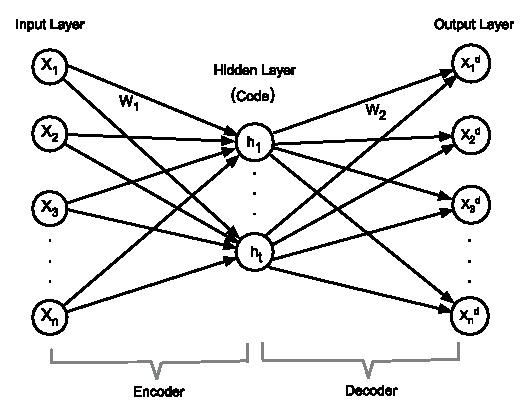
\includegraphics[width=.75\textwidth]{chapters/utility/img/ae_schema.eps}
\caption{Classical structure of an autoencoder. $X$ is the input data of the input layer, $h$ is the hidden layer's data, and $X^d$ is the reconstructed output data in the output layer.}
\label{fig:vae:ae_schema}
\end{figure}

\begin{lvae}

Recalling \autoref{ch:vae}, the essence of a variational autoencoder is that we take a variational distribution $q_\phi$ and choose the parameters $\phi$ to fit best the proposed distribution $p(\bZ)$. We also fit the data likelihood to best reconstruct the input from the proposed latent space distribution. The loss is the variational lower bound, given by
\begin{equation}
\Ls(\theta,\phi;\bX,\bA)=-D_{KL}(q_\phi(\bZ|\bX,\bA), p_\theta(\bZ))+\mathbb{E}_{q_\phi}\left[\log p_\theta(\bA|\bZ)\right]
\end{equation}

\end{lvae}
